\documentclass[11pt]{article}

\usepackage[english]{babel}
\usepackage[utf8]{inputenc}
\usepackage[T1]{fontenc}
\usepackage{lmodern}
\usepackage{microtype}
\usepackage{amsmath,amssymb,amsthm,mathtools,amscd}
\usepackage[a4paper,margin=1in]{geometry}
\usepackage{parskip}
\usepackage{enumitem}
\usepackage{xcolor}
\usepackage{hyperref}
\usepackage{tikz}
\usetikzlibrary{arrows.meta,positioning,fit,calc,backgrounds}

\hypersetup{colorlinks=true,linkcolor=blue,citecolor=blue,urlcolor=blue}

\newcommand{\R}{\mathbb{R}}
\newcommand{\Z}{\mathbb{Z}}
\newcommand{\Q}{\mathbb{Q}}
\newcommand{\kk}{\Bbbk}
\newcommand{\TAMER}{\textsc{TAMER-OP}}
\newcommand{\multipers}{\textsc{multipers}}
\newcommand{\bbb}[1]{\mathbb{#1}}

\newtheorem{theorem}{Theorem}
\newtheorem{proposition}[theorem]{Proposition}
\newtheorem{lemma}[theorem]{Lemma}
\theoremstyle{definition}
\newtheorem{defn}[theorem]{Definition}
\theoremstyle{remark}
\newtheorem*{remark}{Remark}

%%%%%%%%%%%%%%%%%%%%%%%%%%%%%%%%%%%%%%%%%%%%%%%%%%%%%%%%%%%%%%%%%%%%%%%%%%%%%%%%%%%%%%%%%%%%%%%%%%%%%%%%%%%%%%%%%%
%Some formatting tidbits for margins, paragraphs, and removing orphans

% make widows and orphans rare
\clubpenalty =10000
\widowpenalty =10000

% formatting of paragraphs and separation
\setlength{\parindent}{0pt}
\setlength{\parskip}{5pt plus 1pt}
\setlength{\headheight}{13.6pt}

\setlength\marginparwidth{2.2in}
\setlength\marginparsep{1mm}

%%%%%%%%%%%%%%%%%%%%%%%%%%%%%%%%%%%%%%%%%%%%%%%%%%%%%%%%%

\title{Implementation and Ramifications of TAMER-OP: a Toolkit for Algebraic Module Encodings over $\mathbb{R}^n$ and Other Posets}
\author{Erik Mendes Novak}

\date{\today}

\begin{document}
\maketitle
\tableofcontents

\newpage

\section{Introduction}\label{sec:introduction}

Persistent homology is most useful when it converts filtered geometric data into algebraic objects that are simultaneously expressive and computable. In the one-parameter setting these two sides align particularly well. A filtration indexed by a total order gives rise to a persistence module whose structure is rigid enough to admit interval-type decompositions, barcode summaries, and stable diagrammatic invariants \cite{ELZ02,CEH07,CB15,EH10}. In several parameters, however, this balance breaks down. The indexing poset is no longer a chain, a barcode classification is no longer possible in general, and the cost of direct algebraic manipulation grows quickly with the size and geometry of the parameter space \cite{CZ09,Les15,CDSGO16,Oud15}. Multiparameter persistence therefore forces a design choice: one can either work primarily with summary invariants adapted to specific tasks, or one can try to preserve a richer internal algebraic model on which broader constructions remain possible.

The software library \TAMER{} is specifically concerned with the second viewpoint. Its central principle is that the decisive computational move is not a particular invariant, nor a particular data structure for one family of modules, but rather the explicit construction of a finite encoding. Starting from raw data, finite-poset presentations, flange presentations over $\Z^n$, or piecewise-linear presentations over $\R^n$, \TAMER{} first compresses the ambient parameter poset into a finite encoding poset $P$ together with a classifier or encoding map $\pi$. The original object is then represented by a finite-poset module, together with pushed-down presentation data on $P$. Once this finite internal model has been built, the rest of the library's toolkit becomes uniformly available: module morphisms, kernels and cokernels, indicator resolutions, derived functors, rank- and slice-based invariants, serialization, featurization, and visualization can all be performed against the same encoded object. In this sense, encoding is not merely preprocessing, but indeed is the organizing principle of the entire system.

This viewpoint is directly motivated by Miller's theory of tame modules over posets \cite{Mil20}. Miller's framework shows that, under appropriate finiteness hypotheses, several apparently different descriptions of a module are equivalent: finite encodings, indicator presentations by upsets and downsets, and indicator resolutions all express the same controlled form of tameness. That equivalence extends from the theoretical to a strong implementation consequence. Rather than building separate pipelines for geometric data, algebraic summaries, and downstream statistics, one can work to make the encoding step explicit and robust, and then treat the encoded module as the shared internal object from which all later computations are derived.

\TAMER{} consequently accordingly advances three intertwined claims. Firstly, the finite-encoding perspective provides a mathematically coherent bridge between large ambient parameter spaces and finite combinatorial models. Secondly, this bridge is sufficiently explicit to support a unified software architecture that begins with multiple front end representations and data-ingestion pipelines, and ends with exact algebraic, invariant, and statistical workflows. Thirdly, this architecture is practical, as it supports tractable computation on data sets of ordinary scientific scale and is computationally competitive against existing multiparameter persistence libraries where there is implementation overlap.

In the remainder of this thesis, we first introduce the mathematical machinery behind multiparameter persistence, enough to understand what its difficulties are. Then, we show how tame modules present a computational solution. Then, we overview \TAMER{}, from the front end input, to the encoding step, to the downstream computations that are made possible due to it. Finally, we benchmark the library to demonstrate its tractability. This order is deliberate; we hope to demonstrate that nearly every distinctive feature of the library is best understood as more than just an isolated implementation trick, and indeed as a consequence of making the finite encoding step explicit and central.



\section{Multiparameter persistence and its difficulties}\label{sec:background}

Persistent homology begins with a filtered topological object and produces algebra. One chooses an indexing poset, usually a subset of $\R^d$ or $\Z^d$ with the coordinatewise order, and records a vector space at each parameter value together with linear maps along the order relation. In one parameter, this construction leads to a theory with a very strong structure theorem. In several parameters, the same definition still makes sense, but the structure theory changes completely. The purpose of this section is to introduce the basic language carefully and to explain why the multiparameter case resists the sort of complete description that is available in one parameter. Throughout, let $\kk$ be a field.

\subsection{Posets, filtrations, and persistence modules}

The correct indexing objects in persistence theory are partially ordered sets. A poset may be viewed as a category, and a persistence module is then just a functor out of that category.

\begin{defn}[Poset]
A \emph{partially ordered set} is a set $Q$ together with a relation $\leq$ that is reflexive, antisymmetric, and transitive.
\end{defn}

\begin{defn}[A poset as a category]
Given a poset $(Q,\leq)$, one forms a small category, again denoted $Q$, whose objects are the elements of $Q$, and such that there is a unique morphism $q \to q'$ if and only if $q \leq q'$. Composition is forced by transitivity and identity morphisms are forced by reflexivity.
\end{defn}

A category of this form is thin: between any two objects there is at most one morphism. This observation is what allows order theory and homological algebra to interact in persistence.

\begin{defn}[$Q$-module, or persistence module]
Let $Q$ be a poset and let $\mathbf{Vect}_{\kk}$ denote the category of vector spaces over $\kk$. A \emph{$Q$-module} is a covariant functor
\[
M : Q \longrightarrow \mathbf{Vect}_{\kk}.
\]
Equivalently, one specifies a vector space $M(q)$ for each $q \in Q$ and, for each comparable pair $q \leq q'$, a linear map
\[
M(q \leq q') : M(q) \to M(q')
\]
subject to the functoriality relations
\[
M(q \leq q)=\mathrm{id}_{M(q)}, \qquad
M(q \leq q'') = M(q' \leq q'') \circ M(q \leq q')
\]
whenever $q \leq q' \leq q''$.
\end{defn}

A morphism $f : M \to N$ of $Q$-modules is a natural transformation. Concretely, this means that for each $q \in Q$ there is a linear map $f_q : M(q) \to N(q)$ and, for each $q \leq q'$, the square
\[
\begin{CD}
M(q) @>{M(q\leq q')}>> M(q')\\
@V{f_q}VV @VV{f_{q'}}V\\
N(q) @>{N(q\leq q')}>> N(q')
\end{CD}
\]
commutes.

The persistent homology modules arising from filtered topology fit into this framework in the most direct possible way: if $\mathcal{F} : Q \to \mathbf{Top}$ is a filtration, then for each homological degree $i$ one obtains a $Q$-module
\[
H_i(\mathcal{F};\kk) : Q \longrightarrow \mathbf{Vect}_{\kk}
\]
by functoriality of homology.

The category of $Q$-modules inherits the basic exact structure of $\mathbf{Vect}_{\kk}$.

\begin{proposition}[Pointwise abelian structure]
For any small category $\mathcal{C}$, the functor category $\mathrm{Fun}(\mathcal{C},\mathbf{Vect}_{\kk})$ is abelian. In particular, when $\mathcal{C}=Q$ is a poset, kernels, cokernels, images, and coimages are computed pointwise \cite{Mac98,Wei94}.
\end{proposition}

This pointwise abelian structure is the key to computational feasibility. If the indexing poset is finite, then a persistence module is represented by finitely many vector spaces and finitely many structure maps, so abelian constructions reduce to finite linear algebra. If the indexing poset is infinite, the same proposition still holds formally, but it does not provide a usable algorithm. This gap between formal exactness and finite computability is the problem that motivates the encoding viewpoint later in the thesis.

\subsection{The one-parameter scope}

The one-parameter theory is the model initial case. Let $Q$ be $\R$ or $\Z$ with the usual total order. Then persistent homology produces modules indexed by a chain, and that special geometry forces a rigid structure theory.

\begin{defn}[Interval module]
Let $I \subseteq \R$ be an interval. The associated \emph{interval module} $\kk_I$ is defined by
\[
\kk_I(t)=
\begin{cases}
\kk, & t \in I,\\
0, & t \notin I,
\end{cases}
\]
with structure maps equal to the identity whenever both source and target lie in $I$, and equal to the zero map otherwise.
\end{defn}

\begin{theorem}[Barcode decomposition]
Under the usual pointwise-finite and local-finiteness hypotheses from persistence theory, a one-parameter persistence module decomposes as a direct sum of interval modules, uniquely up to isomorphism and reordering of summands \cite{CB15,Oud15}.
\end{theorem}

This theorem explains why barcodes are so effective. In the one-parameter setting they are more than just heuristic pictures, indeed encoding the module itself under the standard finiteness assumptions. Stability theory then shows that the associated persistence diagrams vary continuously under perturbation of the filtered data \cite{ELZ02,CEH07,CDSGO16}. Thus one-parameter persistence enjoys both classification and stability.

That combination does not generalize. It is natural to ask for the same story in several parameters, but already the algebra of the indexing category becomes too rich.

\subsection{What changes in several parameters}

For $d \geq 2$, the standard indexing posets are $\Z^d$ or $\R^d$ with the coordinatewise order
\[
a \leq b \quad \Longleftrightarrow \quad a_i \leq b_i \text{ for all } i.
\]
This change from a chain to a partial order has major consequences. For example, there are now many incomparable pairs. A module is no longer controlled by a single linear progression of births and deaths. Additionally, if one works over $\Z^d$ or $\mathbb{N}^d$, the algebra is equivalent to the algebra of multigraded modules over a polynomial ring.

\begin{proposition}[Algebraic model over $\mathbb{N}^d$]
A persistence module indexed by $\mathbb{N}^d$ is equivalent to an $\mathbb{N}^d$-graded module over the polynomial ring $\kk[x_1,\dots,x_d]$, where multiplication by $x_i$ records the structure map in the $i$th coordinate direction \cite{CZ09,Oud15}.
\end{proposition}

This equivalence is powerful, because it brings in multigraded commutative algebra. It is also, however, the source of the difficulty. The polynomial ring in several variables is not a principal ideal domain, multigraded modules need not decompose into interval modules, and indecomposables occur in families rather than as a discrete list. In particular, the multiparameter theory does not admit a barcode theorem comparable to the one-parameter case \cite{CZ09,Les15}.

So the obstruction is not just that computations become larger. The problem is also structural: in one parameter, the module itself can be packaged into a complete discrete invariant; but, in several parameters, there is in general no analogous finite complete invariant of that simple form.

This has two immediate consequences for computation.

\begin{enumerate}[label=(\roman*)]
    \item One should not expect a universal normal form that is both complete and as easy to manipulate as a barcode.
    \item If one wants to preserve the full algebraic object, rather than only a summary of it, then one needs a different notion of finiteness.
\end{enumerate}

That second point is the central issue addressed by \TAMER{}. The relevant question is not how to force the multiparameter theory back into one-parameter language, but how to represent the module by finite, computable data without dismissing the algebra one later wants to use.

\subsection{What one computes in place of a barcode}

Although there is no complete barcode-like invariant in general, several families of invariants remain useful. They are partial by necessity, each only recording one aspect of the module rather than all of it. We now overview some main ones.

\begin{defn}[Rank invariant]
Let $M$ be a $Q$-module. For each comparable pair $a \leq b$ in $Q$, the \emph{rank invariant} is
\[
\rho_M(a,b) = \operatorname{rank}\bigl(M(a \leq b)\bigr).
\]
\end{defn}

The rank invariant records how much information survives from one parameter value to another. In one parameter it determines the barcode. In several parameters it remains important, but is no longer a complete characterization (different modules may have the same rank invariant).

A second common idea is to probe a multiparameter module along one-dimensional subposets.

\begin{defn}[Restriction to a chain or slice]
If $\lambda : Q' \to Q$ is a monotone map, then the pullback
\[
\lambda^* M := M \circ \lambda
\]
is a $Q'$-module. When $Q'$ is totally ordered, $\lambda^*M$ is an ordinary one-parameter persistence module. Its barcode is then called a \emph{slice barcode} or \emph{fibered barcode}, depending on the context.
\end{defn}

This recovers the successful one-parameter theory on each slice, and it is the basis of tools such as RIVET \cite{LW15,RIVET}. But again, different multiparameter modules can have the same family of one-dimensional restrictions.

There are also dimension-based invariants. The most basic one is the restricted Hilbert function
\[
q \longmapsto \dim_{\kk} M(q).
\]
This records the size of each fiber but not the structure maps between fibers.

A related family comes from chain complexes rather than from a single module. If $C^\bullet$ is a chain or cochain complex of modules on a finite encoding poset, one may define the Euler characteristic function
\[
\chi_C(q) = \sum_t (-1)^t \dim_{\kk} C^t(q).
\]
When $C^\bullet$ arises from filtered topology, this agrees with the alternating sum of the homology dimensions at $q$. In this thesis, when we speak of \emph{Euler invariants}, we mean invariants built from this Euler characteristic function, together with the finite-grid signed measures obtained from it by Mobius inversion. These invariants are useful because they are cheap to evaluate, easy to visualize, and often effective in statistical pipelines, even though they are far from complete.

The essential point is that none of these constructions replaces the module itself. Rank invariants, slice barcodes, Hilbert functions, and Euler characteristic functions are all informative, but each forgets some part of the structure. This is why the central focus of \TAMER{} is not the design of a single invariant, but rather the construction of a finite algebraic model from which many different invariants and constructions can be extracted.

\section{Tameness, finite encodings, and computability}\label{sec:tameness}

The correct response to the loss of barcode classification is to identify a class of modules that still admit finite descriptions and remain amenable to exact algebraic computation. In this thesis that role is played by tame modules in the sense of Miller \cite{Mil20}. We now explore what finite encodings are and why tameness is so important.

\subsection{Finite encodings}

The basic finiteness notion is that a module factors through a finite poset.

\begin{defn}[Finite encoding]
Let $Q$ be a poset and let $M$ be a $Q$-module. A \emph{finite encoding} of $M$ consists of
\begin{enumerate}[label=(\roman*)]
    \item a finite poset $P$,
    \item a monotone map $\pi : Q \to P$, and
    \item a $P$-module $H$ with finite-dimensional stalks,
\end{enumerate}
such that
\[
M \cong \pi^* H = H \circ \pi.
\]
\end{defn}

Here $\pi^*$ denotes pullback along the poset morphism $\pi$.

\begin{defn}[Pullback along a poset morphism]
If $\pi : Q \to P$ is monotone and $H$ is a $P$-module, the \emph{pullback} of $H$ along $\pi$ is the $Q$-module
\[
\pi^*H := H \circ \pi.
\]
Thus
\[
(\pi^*H)(q)=H(\pi(q))
\]
for each $q \in Q$, and the structure map from $q$ to $q'$ is the structure map of $H$ from $\pi(q)$ to $\pi(q')$.
\end{defn}

\begin{proposition}[Exactness of pullback]
For any monotone map $\pi : Q \to P$, the pullback functor
\[
\pi^* : \mathbf{Vect}_{\kk}^{P} \longrightarrow \mathbf{Vect}_{\kk}^{Q}
\]
is exact.
\end{proposition}

\begin{proof}
Kernels, cokernels, and finite direct sums in a functor category are computed pointwise. Pullback by precomposition simply evaluates the $P$-module at $\pi(q)$ instead of at $q$, so exactness is preserved at every stalk.
\end{proof}

A finite encoding is therefore not a lossy statistic. It is an isomorphic re-expression of the module through a finite index category. If $M \cong \pi^*H$, then the algebraic behavior of $M$ is constant on each fiber of $\pi$, and every fiber and structure map of $M$ is recovered from the finite-poset module $H$ together with the map $\pi$.

\subsection{Tame modules and tame morphisms}

With the notion of finite encoding in hand, tameness is simple to state.

\begin{defn}[Tame module]
Let $Q$ be a poset. A $Q$-module $M$ is \emph{tame} if it admits a finite encoding.
\end{defn}

This definition is stronger than merely asking for finite-dimensional fibers or finite-rank structure maps. It requires the entire module to be controlled by finitely many regions of parameter space. That extra strength is exactly what makes it suitable for computation.

There is, however, a subtle categorical point. If one allows all natural transformations between tame modules, kernels and cokernels need not remain finitely encoded. The correct category is obtained by restricting to morphisms that are themselves compatible with a common finite description.

\begin{defn}[Tame morphism]
Let $M$ and $N$ be tame $Q$-modules. A morphism $f : M \to N$ is called \emph{tame} if there exists a common finite constant subdivision, or equivalently a common finite encoding context, in which the component maps of $f$ are constant on each region in the obvious sense \cite{Mil20}.
\end{defn}

\begin{theorem}[Miller]
With tame modules as objects and tame morphisms as morphisms, the resulting category is abelian \cite{Mil20}.
\end{theorem}

This addresses a natural concern. One might worry that finite encodability is too restrictive to support genuine homological algebra. The point of Miller's framework is that this is not the case: the correct category of tame modules is still abelian, so kernels, cokernels, exact sequences, and derived constructions remain available. Recent work of Waas further clarifies that categories of finitely encodable persistence modules have better exact behavior than one might first expect, reinforcing the view that finite encodability is a mathematically natural rather than ad hoc hypothesis \cite{Waa24}.

Thus, the word tame should not be read as a purely artificial restriction imposed for software convenience. It identifies the point at which an ambient persistence module can be represented by finite data without collapsing to a summary invariant that loses information. For the purposes of \TAMER{}, tameness is the hypothesis that makes it possible to keep the module, rather than discard it, and still work computationally. 

\subsection{Upsets, downsets, and fringe presentations}

Finite encodings are one language for tameness. Another is given by indicator modules attached to order-theoretic regions.

\begin{defn}[Upsets and downsets]
Let $Q$ be a poset.
\begin{enumerate}[label=(\roman*)]
    \item An \emph{upset} is a subset $U \subseteq Q$ such that $q \in U$ and $q \leq q'$ imply $q' \in U$.
    \item A \emph{downset} is a subset $D \subseteq Q$ such that $q' \in D$ and $q \leq q'$ imply $q \in D$.
\end{enumerate}
For $q \in Q$, the corresponding principal upset and principal downset are
\[
\uparrow q = \{q' \in Q : q \leq q'\}, \qquad
\downarrow q = \{q' \in Q : q' \leq q\}.
\]
\end{defn}

\begin{defn}[Indicator modules]
To an upset $U \subseteq Q$ one associates the \emph{upset indicator module} $\kk\{U\}$, defined by
\[
\kk\{U\}(q)=
\begin{cases}
\kk, & q \in U,\\
0, & q \notin U,
\end{cases}
\]
with the evident structure maps. Dually, a downset $D$ determines a \emph{downset indicator module} $\kk\{D\}$.
\end{defn}

On a finite poset, principal upset indicators play the role of indecomposable projective modules, and principal downset indicators play the role of indecomposable injective modules. This is why they are the correct basic pieces for exact algebra on finite posets.

\begin{defn}[Finite fringe presentation]
A \emph{finite fringe presentation} of a $Q$-module $M$ consists of a morphism
\[
\varphi : \bigoplus_{i=1}^m \kk\{U_i\} \longrightarrow \bigoplus_{j=1}^r \kk\{D_j\}
\]
from a finite direct sum of upset indicator modules to a finite direct sum of downset indicator modules such that $M \cong \operatorname{im}(\varphi)$ \cite{Mil20}.
\end{defn}

This presentation language is one of the key bridges between geometry and algebra in the library. Upsets encode where generators are born and persist upward in the order; downsets encode where relations become enforced; and the matrix of $\varphi$ records how these pieces interact.

\subsection{Why encoding is the right answer}

The key fact is that tameness admits several equivalent finite descriptions.

\begin{theorem}[Syzygy theorem, after Miller]
For a module over a poset, the following finiteness conditions are equivalent: existence of a finite encoding, existence of a finite fringe presentation, and existence of finite resolutions by indicator modules \cite{Mil20}.
\end{theorem}

This theorem explains why encoding is the right computational answer to the difficulties of multiparameter persistence. We describe three consequences of it now.

Firstly, it says that one does not need to choose between a geometric region picture, a presentation by births and deaths, and a homological description by resolutions. For tame modules, these are different finite views of the same object.

Secondly, it explains what is gained by encoding. We do not package a multiparameter module back into one clean barcode, because that is impossible in general. Instead, we pass to a finite poset on which the module is represented exactly by finite data. Once that finite representation has been constructed, one can carry out actual algebra: kernels, cokernels, change-of-poset operations, indicator resolutions, and derived functor calculations. Invariants such as rank functions, slice barcodes, Hilbert functions, Euler characteristic functions, and their associated signed measures are then extracted from this finite model, rather than substituted for it.

Thirdly, it explains why this approach does not lose information in the sense relevant to the library. The encoded module on the finite poset is not a secondary summary attached to the original module, but rather the finite algebraic object through which the original module is being represented. The purpose of the encoding step is therefore not compression for its own sake. It is to move from an ambient indexing space that is too large for direct exact computation to a finite model on which exact computation is possible.

This is the perspective adopted throughout the rest of the thesis. The next section therefore begins with the architecture of the encoding-centered system itself, because once the encoded finite-poset module has been built, the rest of the library follows from that choice.

\section{Overview of \TAMER{} as an encoding-centered system}\label{sec:system-overview}

The previous section explained why finite encodings are mathematically legitimate and computationally necessary.  This section explains how that idea informs the organization of \TAMER{}.  We identify the stable mathematical interfaces that the implementation is built around; these are arranged so that many front-end objects feed a single encoding step, and that encoding step in turn feeds many downstream computations.

\subsection{The main pipeline}

At the highest level, the library is organized around the composite workflow
\[
\mathcal{I}
\xrightarrow{\ \mathsf{prepare}\ }
\mathcal{P}
\xrightarrow{\ \mathsf{encode}\ }
\mathcal{E}
\xrightarrow{\ \mathsf{analyze}\ }
\mathcal{O},
\]
where:
\begin{itemize}[leftmargin=1.5em]
    \item $\mathcal{I}$ denotes raw inputs, such as data files, point clouds, graphs, images, or already structured presentation objects;
    \item $\mathcal{P}$ denotes pre-encoding mathematical objects, such as finite fringe modules, flanges over $\mathbb{Z}^n$, PL or box presentations over $\mathbb{R}^n$, and graded complexes produced by ingestion;
    \item $\mathcal{E}$ denotes finite encodings, represented concretely by a finite poset together with an encoded module and the maps needed to interpret it back in the ambient parameter space; and
    \item $\mathcal{O}$ denotes downstream outputs, including categorical constructions, derived functors, invariants, feature vectors, serialized artifacts, and visual objects.
\end{itemize}

The crucial middle object $\mathcal{E}$ is what the codebase packages as an \texttt{EncodingResult}.  Stripping away software metadata, the mathematical content of such an object is the tuple
\[
(P,M,\pi,H).
\]
Here $P$ is a finite encoding poset, $M$ is a finite-poset module on $P$, $\pi$ is the classifier or encoding map from the ambient domain to $P$, and $H$ is a pushed-down fringe presentation when such a presentation is available.  Not every later calculation uses all four pieces, but together they constitute the canonical object available to the rest of the system.

This packaging is contextually important: the encoding step does not merely return a poset and forget how it arose; it returns a finite module, a mechanism for point location in the original parameter space, and enough provenance to support comparison, serialization, and visualization. From the user-facing point of view, this is the moment at which a raw front end object becomes a reusable algebraic object.

Figure~\ref{fig:system-overview} summarizes the resulting architecture.

\begin{figure}[h]
\centering
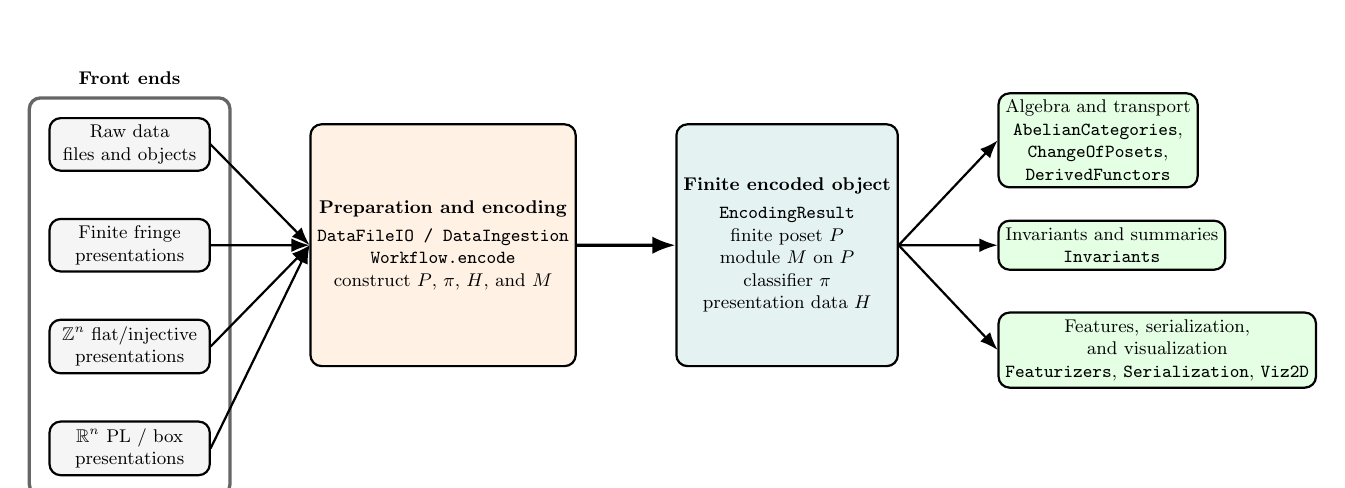
\begin{tikzpicture}[
    >=Latex,
    scale=0.74,
    transform shape,
    node distance=8mm and 10mm,
    every node/.style={font=\small},
    src/.style={rounded corners, draw, thick, align=center, minimum width=2.75cm, minimum height=0.8cm, fill=gray!8},
    stage/.style={rounded corners, draw, thick, align=center, minimum width=3.8cm, minimum height=1.0cm, fill=orange!10},
    outbox/.style={rounded corners, draw, thick, align=center, minimum width=3.0cm, minimum height=0.82cm, fill=green!10},
    layer/.style={rounded corners, draw=black!60, very thick, inner sep=7pt}
]

\node[src] (raw) {Raw data\\files and objects};
\node[src, below=of raw] (finite) {Finite fringe\\presentations};
\node[src, below=of finite] (flange) {$\mathbb{Z}^n$ flat/injective\\ presentations};
\node[src, below=of flange] (pl) {$\mathbb{R}^n$ PL / box\\presentations};
\node[layer, fit=(raw)(finite)(flange)(pl), label={[yshift=0.2em]above:\textbf{Front ends}}] {};

\node[stage, right=17mm of finite, minimum height=4.15cm] (encode) {
\textbf{Preparation and encoding}\\[0.3em]
\texttt{DataFileIO / DataIngestion}\\
\texttt{Workflow.encode}\\
construct $P$, $\pi$, $H$, and $M$
};

\node[stage, right=17mm of encode, minimum height=4.15cm, fill=teal!10] (result) {
\textbf{Finite encoded object}\\[0.3em]
\texttt{EncodingResult}\\
finite poset $P$\\
module $M$ on $P$\\
classifier $\pi$\\
presentation data $H$
};

\node[outbox, right=17mm of result, yshift=18mm] (alg) {Algebra and transport\\\texttt{AbelianCategories},\\\texttt{ChangeOfPosets},\\\texttt{DerivedFunctors}};
\node[outbox, right=17mm of result] (inv) {Invariants and summaries\\\texttt{Invariants}};
\node[outbox, right=17mm of result, yshift=-18mm] (feat) {Features, serialization,\\and visualization\\\texttt{Featurizers}, \texttt{Serialization}, \texttt{Viz2D}};

\draw[->, thick] (raw.east) -- (encode.west);
\draw[->, thick] (finite.east) -- (encode.west);
\draw[->, thick] (flange.east) -- (encode.west);
\draw[->, thick] (pl.east) -- (encode.west);
\draw[->, very thick] (encode.east) -- (result.west);
\draw[->, thick] (result.east) -- (alg.west);
\draw[->, thick] (result.east) -- (inv.west);
\draw[->, thick] (result.east) -- (feat.west);

\end{tikzpicture}
\caption{A system-level view of \TAMER.  Multiple front ends are normalized into a single encoded object, and all later computation branches from that encoded object rather than from the original ambient representation.}
\label{fig:system-overview}
\end{figure}

The diagram is purposefully thin in the center but branched in input and output.  The left side is diverse because the library is intended to accept front-end objects in the form most natural to their source.  The middle is narrow because there is only one conceptual move that matters: build a finite encoding.  The right side branches again because, once the encoded object exists, many different computational goals can be pursued from the same internal representation.

This thin diagrammatic section characterizing encoding identifies the precise place at which the computational problem changes style. Before encoding, one is still dealing with ambient parameter spaces, geometric representations, filtration choices, and presentation-specific subtleties.  After encoding, one is dealing with a finite-poset module.  The post-encoding world is therefore uniform even though the pre-encoding world is intentionally heterogeneous.

This is also the main mathematical reason that \TAMER{} can do things that are awkward or impossible for existing libraries, which are generally built around architectures that prioritize only summaries and invariants.  Once an actual encoded module has been retained, one may compute kernels, cokernels, equalizers, pushouts, projective and injective approximations, derived functors, and comparison transports before one ever decides which invariant or feature vector to extract.  The encoded module is therefore not just a transient intermediate artifact, but the central object around which the rest of the pipeline is organized.

\subsection{Architectural layering}

The flow chart of figure \ref{fig:system-overview} represents the curated user experience, but to orchestrate that in \TAMER{} we designed a layered architecture that separates code files based on use, with each layer building on the abstractions introduced by the previous one.

At the bottom lies a runtime and linear-algebra layer.  The role of this layer is to provide exact and backend-aware matrix kernels, together with caches and autotuned thresholds, so that later algebraic code can be written at the level of modules rather than at the level of ad hoc numerical special cases.  In the present codebase this role is played chiefly by the \texttt{CoreModules} and \texttt{FieldLinAlg} file families.

Above that lies the finite-poset representation layer.  This is the layer in which finite posets, upsets, downsets, fringe modules, finite-poset modules, abelian-category constructions, and indicator resolutions are represented concretely.  Conceptually, this is the algebraic core of the system.  Once an object is being expressed by this layer, ordinary linear algebra and functor algebra can be applied directly.  The files \texttt{FiniteFringe}, \texttt{Modules}, \texttt{AbelianCategories}, and \texttt{IndicatorResolutions} occupy this level.

The encoding layer sits above the representation layer and below the user-facing workflow.  Its job is to build finite region posets and classifier maps from front-end objects over $\mathbb{Z}^n$ or $\mathbb{R}^n$, together with any compiled or cached structures needed for efficient point location and pushforward.  This is where the library's main differentiating algorithms live.  In the current codebase, the relevant file families are \texttt{EncodingCore}, \texttt{ZnEncoding}, \texttt{PLBackend}, and \texttt{PLPolyhedra}.

Then comes the orchestration layer.  Rather than exposing every internal constructor directly to ordinary users, \TAMER{} organizes common workflows through a small number of stable entry points.  The key example is \texttt{Workflow.encode}, which converts a front-end object into an \texttt{EncodingResult}.  Similar wrappers then dispatch to homological algebra, invariants, and comparison routines.  The \texttt{EncodingResult} object is important here because it carries not only the encoded mathematical object but also options, provenance, backend choice, and metadata.

Finally, several cross-cutting layers operate in parallel with the main algebraic pipeline.  The data ingestion layer bridges raw data and formal presentations.  The serialization layer makes front ends, encodings, and feature artifacts reproducible.  The featurization layer treats encoded modules as reusable objects in statistical and machine-learning workflows.  The visualization layer treats the same encoded objects as the basis for exploration and explanation.  These are more than just auxiliary conveniences added after the mathematical design was fixed, they are part of what it means for the encoded module to serve as a stable internal language across the whole system.

This layering does not follow the design of the flow-chart in figure \ref{fig:system-overview}, but ensures extensible software development and works in tandem to the conceptual user experience design. However, the rest of the thesis will follow the flow of figure \ref{fig:system-overview} again (ultimately, that conceptualization of the library is the most expressive for users), with the next chapter describing pre-encoding objects and data interfaces.


\section{Pre-encoding objects and data interfaces}\label{sec:pre-encoding}

Sections~\ref{sec:background} and~\ref{sec:tameness} introduced the mathematical reason that a finite encoding should exist and should be the object on which exact computation is carried out.  Before one can build such an encoding, however, one needs a finite front end description of the module to be encoded.  This chapter describes the principal front ends accepted by \TAMER{}.

The guiding principle is as follows: the library is intentionally permissive about the form in which a module is first described, but intentionally strict about the object on which later algebra is done.  On the input side, one may begin with a module already indexed by a finite poset, with a \(\mathbb{Z}^n\)-presentation adapted to finitely determined modules, with a piecewise-linear presentation over \(\R^n\), or with raw topological data from which such a presentation can be constructed.  On the output side of the encoding step there is only the working language of a module on a finite encoding poset.

\subsection{Finite-poset presentations: finite fringe presentations and indicator data}

The simplest front end occurs when the indexing poset is already finite.  In that case no geometric compression is needed to obtain a finite combinatorial object, and the basic question is only how to package the module in a form that is easy to manipulate and easy to compare with later encoded outputs.

Let \(P\) be a finite poset.  As in Section~\ref{sec:tameness}, an upset \(U \subseteq P\) determines an indicator module \(\kk\{U\}\), and a downset \(D \subseteq P\) determines an indicator module \(\kk\{D\}\).  Since \(P\) is finite, these indicator modules are themselves finite diagrams of finite-dimensional vector spaces.

\begin{defn}[Finite fringe presentation on a finite poset]
	Let \(P\) be a finite poset and let \(\kk\) be a field.  A \emph{finite fringe presentation} on \(P\) consists of finitely many upsets \(U_1,\dots,U_m\subseteq P\), finitely many downsets \(D_1,\dots,D_r\subseteq P\), and a morphism
	\[
	\varphi : \bigoplus_{i=1}^m \kk\{U_i\}\longrightarrow \bigoplus_{j=1}^r \kk\{D_j\},
	\]
	with the associated module defined as
	\[
	M:=\operatorname{im}(\varphi).
	\]
	Equivalently, once bases are chosen on the one-dimensional indicator summands, the presentation is specified by a matrix
	\[
	\Phi\in \kk^{r\times m}
	\]
	subject to the support condition that \(\Phi_{ji}=0\) whenever \(U_i\cap D_j=\varnothing\).
\end{defn}

The matrix description is especially concrete on a finite poset.  For each vertex \(p\in P\), define the active column and row sets
\[
I(p)=\{i\in\{1,\dots,m\}:p\in U_i\},
\qquad
J(p)=\{j\in\{1,\dots,r\}:p\in D_j\}.
\]
Evaluating the presentation at \(p\) yields a linear map
\[
\varphi_p : \kk^{I(p)}\longrightarrow \kk^{J(p)}
\]
whose matrix is the submatrix \(\Phi_{J(p),I(p)}\).  Thus the fiber at \(p\) is
\[
M(p)=\operatorname{im}(\varphi_p),
\qquad
\dim_\kk M(p)=\operatorname{rank}(\Phi_{J(p),I(p)}).
\]
In other words, the module is read off from the same finite matrix together with the membership pattern of each vertex in the chosen upsets and downsets.

This front end matters for two central reasons.  Firstly, it is the cleanest correctness model in the whole library.  When the user already knows the finite indexing poset, there is no mystery with the encoding; all later kernels, cokernels, Hom, Ext, and invariant computations can be checked directly against this finite presentation.  Secondly, finite fringe presentations are also the natural output of the encoding step, not just merely one among many input formats.  The point of encoding is precisely to replace a module on a large poset by a finite-poset module or, equivalently, by a finite fringe presentation on a finite region poset.  For that reason the finite fringe language is both a front end description and the simplest model of the finite encoding.

\subsection{$\mathbb{Z}^n$ front end: flange presentations and finitely determined data}

The next front end is adapted to modules over \(\mathbb{Z}^n\) with the coordinatewise order.  This is the natural discrete setting for many multifiltration constructions, and it is also the setting in which the connection with multigraded commutative algebra is most direct \cite{CZ09}.  A \(\mathbb{Z}^n\)-module is a functor from the poset category \(\mathbb{Z}^n\) to vector spaces, equivalently a multigraded representation with structure maps in the positive coordinate directions.

A particularly important class is formed by finitely determined modules.

\begin{defn}[Finitely determined \(\mathbb{Z}^n\)-module]
	A \(\mathbb{Z}^n\)-module \(M\) is \emph{finitely determined} if there exists \(a\in \mathbb{Z}^n\) such that for every \(b\geq a\) and every standard basis vector \(e_i\), the structure map
	\[
	M(b\leq b+e_i) : M(b)\longrightarrow M(b+e_i)
	\]
	is an isomorphism.
\end{defn}

This condition says that, sufficiently far in the positive orthant, the module stops changing in any essential way.  It is the discrete analogue of eventual constancy on regions, and it is one of the standard hypotheses under which finite descriptions become possible.

Miller's theory packages these modules using \emph{flats} and \emph{injectives}.  Fix a subset \(\tau\subseteq \{1,\dots,n\}\), thought of as a set of free coordinate directions, and a lattice point \(b\in \mathbb{Z}^n\).  The corresponding flat and injective regions are
\[
F_{\tau,b}=\{a\in \mathbb{Z}^n: a_i\geq b_i\text{ for every }i\notin \tau\},
\]
\[
E_{\tau,b}=\{a\in \mathbb{Z}^n: a_i\leq b_i\text{ for every }i\notin \tau\}.
\]
The coordinates in \(\tau\) are unrestricted.  Thus principal upsets and principal downsets occur as the special case \(\tau=\varnothing\), while more general choices of \(\tau\) allow one to model affine coordinate flats in the sense used in Miller's \(\mathbb{Z}^n\)-theory \cite{Mil20}.

\begin{defn}[Flange presentation]
	A \emph{flange presentation} over \(\mathbb{Z}^n\) consists of finitely many flats \(F_1,\dots,F_m\), finitely many injectives \(E_1,\dots,E_r\), and a matrix
	\[
	\Phi\in \kk^{r\times m}
	\]
	with the support condition \(\Phi_{ji}=0\) whenever \(F_i\cap E_j=\varnothing\).  It presents the module
	\[
	M:=\operatorname{im}\!\left(\bigoplus_{i=1}^m \kk\{F_i\}\longrightarrow \bigoplus_{j=1}^r \kk\{E_j\}\right).
	\]
\end{defn}

The local behavior is parallel to the finite fringe case.  For a lattice point \(g\in\mathbb{Z}^n\), let
\[
I(g)=\{i:g\in F_i\},\qquad J(g)=\{j:g\in E_j\}.
\]
Then the fiber \(M(g)\) is the image of the submatrix \(\Phi_{J(g),I(g)}\), so fiber dimensions and local maps are determined by the active flats and injectives at \(g\).  What changes, compared to the finite-poset case, is that the ambient poset is infinite.  The flange presentation therefore serves as a compact input language whose membership predicates can be evaluated anywhere in \(\mathbb{Z}^n\), but which is intended to be encoded before more substantial algebra is done.

\subsection{$\mathbb{R}^n$ front-end: PL fringes and box presentations}

For modules over \(\mathbb{R}^n\), one needs a geometric version of the same idea.  The relevant inputs are piecewise-linear upsets and downsets, represented by finite polyhedral data.  This is the correct front end for modules whose behavior changes along finitely many polyhedral boundaries, and it is also the natural setting for geometric constructions arising from stratified topology and sheaf-theoretic viewpoints on persistence \cite{KS18,Mil23}.

\begin{defn}[PL upset and PL downset]
	A \emph{PL upset} in \(\mathbb{R}^n\) is an upward-closed subset that is a finite union of convex polyhedra.  A \emph{PL downset} is defined dually as a downward-closed finite union of convex polyhedra.
\end{defn}

The front end presentation is then the direct real-parameter analogue of a fringe presentation.

\begin{defn}[PL fringe presentation]
	A \emph{PL fringe presentation} over \(\mathbb{R}^n\) consists of finitely many PL upsets \(U_1,\dots,U_m\subseteq\mathbb{R}^n\), finitely many PL downsets \(D_1,\dots,D_r\subseteq\mathbb{R}^n\), and a matrix
	\[
	\Phi\in \kk^{r\times m}
	\]
	with \(\Phi_{ji}=0\) whenever \(U_i\cap D_j=\varnothing\).  The associated module is again the image of the induced morphism
	\[
	\bigoplus_{i=1}^m \kk\{U_i\}\longrightarrow \bigoplus_{j=1}^r \kk\{D_j\}.
	\]
\end{defn}

At a point \(x\in\mathbb{R}^n\), one evaluates the same active-set construction as before,
\[
I(x)=\{i:x\in U_i\},\qquad J(x)=\{j:x\in D_j\},
\]
and the fiber is computed from the submatrix \(\Phi_{J(x),I(x)}\).  Thus the formal algebra is unchanged, with change happening in the geometry of membership and intersection.  In the real setting, a correct implementation must be able to decide whether a point lies in one of the finitely many prescribed polyhedral regions and must be able to identify the induced constant regions of the presentation.

An important specialization is the axis-aligned box backend.  Here one restricts to upsets and downsets of the form
\[
U_{\ell}=\{x\in\mathbb{R}^n:x_i\geq \ell_i\text{ for all }i\},
\qquad
D_u=\{x\in\mathbb{R}^n:x_i\leq u_i\text{ for all }i\}.
\]
This format covers a large and practically relevant class of examples. Additionally, and importantly, they admit a much more direct encoding procedure, covered in the next section. So, ultimately, the polyhedral front end is mathematically more general, while the box front end is algorithmically much simpler, and the library supports both.

\subsection{Raw data, filtrations, and graded complexes}

Not every user begins with a presentation by upsets and downsets.  In topological data analysis the more common starting point is raw data together with a rule for assigning parameter values to cells, simplices, edges, or vertices.  For this reason \TAMER{} includes a data-ingestion layer whose role is to convert raw data into one of the presentation objects discussed above, usually by way of a graded complex.

\begin{defn}[Graded complex]
	Let \(K\) be a finite cell complex.  A \emph{graded complex} over a poset \(Q\) is the data of a grade
	\[
	\deg(\sigma)\in Q
	\]
	for each cell \(\sigma\) of \(K\), subject to the monotonicity condition that if \(\tau\) is a face of \(\sigma\), then
	\[
	\deg(\tau)\leq \deg(\sigma).
	\]
	Equivalently, the chain groups of \(K\) become \(Q\)-graded and the boundary maps are degree-nonincreasing in the usual persistence sense.
\end{defn}

From such a graded complex one obtains persistence modules by taking homology or cohomology degreewise.  In the one-parameter setting this is the standard construction underlying persistent homology \cite{ZC05}; in the multiparameter setting the same principle applies, but the grade now lies in \(\mathbb{Z}^n\), \(\mathbb{R}^n\), or another suitable poset.

The data-ingestion layer accepts several kinds of raw or partially structured input.  The most basic data objects are point clouds, graphs, and images.  In addition, the user may begin with an already constructed graded complex, a multicritical graded complex in which a cell carries several incomparable minimal grades, or a compressed simplex-tree representation of a multifiltered simplicial complex.  The point is not that all of these objects are mathematically identical, but that each of them can be functorially transformed into a graded complex, from which an encoding can then be built.

The transformation is controlled by a typed filtration specification.  For point clouds, representative families include Vietoris--Rips, density-modified Rips, landmark Rips, Delaunay-type, alpha-type, and related constructions.  For graphs, the library supports lower-star, clique lower-star, edge-weighted, geodesic, centrality-based, and other graph-specific filtrations.  For images and cubical data, lower-star and distance-based filtrations play the analogous role.  The output of this stage is still pre-encoding, being a finite graded object with an explicitly recorded parameter assignment, not yet a finite encoding poset.

The next stage of the thesis is to explain how all these front ends we have discussed are converted into a finite encoding poset and a finite module on that poset.



\section{Bibliography notes}\label{app:bibliography-notes}

\begin{thebibliography}{99}

\bibitem[Mil20]{Mil20}
E.~Miller.
\newblock \emph{Homological algebra of modules over posets}.
\newblock \href{https://arxiv.org/abs/2008.00063}{arXiv:2008.00063}, 2020.

\bibitem[Waa24]{Waa24}
L.~Waas.
\newblock \emph{Notes on abelianity of categories of finitely encodable persistence modules}.
\newblock \href{https://arxiv.org/abs/2407.08666}{arXiv:2407.08666}, 2024.

\bibitem[Mil23]{Mil23}
E.~Miller.
\newblock \emph{Stratifications of real vector spaces from constructible sheaves with conical microsupport}.
\newblock \emph{Journal of Applied and Computational Topology}, 7(3):473--489, 2023.
\newblock \href{https://doi.org/10.1007/s41468-023-00112-1}{doi:10.1007/s41468-023-00112-1}.

\bibitem[KS18]{KS18}
M.~Kashiwara and P.~Schapira.
\newblock \emph{Persistent homology and microlocal sheaf theory}.
\newblock \emph{Journal of Applied and Computational Topology}, 2(1--2):83--113, 2018.
\newblock \href{https://arxiv.org/abs/1705.00955}{arXiv:1705.00955}.

\bibitem[CB15]{CB15}
W.~Crawley-Boevey.
\newblock \emph{Decomposition of pointwise finite-dimensional persistence modules}.
\newblock \emph{Journal of Algebra and Its Applications}, 14(5):1550066, 2015.
\newblock \href{https://doi.org/10.1142/S0219498815500668}{doi:10.1142/S0219498815500668}.

\bibitem[ZC05]{ZC05}
A.~Zomorodian and G.~Carlsson.
\newblock \emph{Computing persistent homology}.
\newblock \emph{Discrete \& Computational Geometry}, 33:249--274, 2005.
\newblock \href{https://doi.org/10.1007/s00454-004-1146-y}{doi:10.1007/s00454-004-1146-y}.

\bibitem[CZ09]{CZ09}
G.~Carlsson and A.~Zomorodian.
\newblock \emph{The theory of multidimensional persistence}.
\newblock \emph{Discrete \& Computational Geometry}, 42:71--93, 2009.
\newblock \href{https://doi.org/10.1007/s00454-009-9176-0}{doi:10.1007/s00454-009-9176-0}.

\bibitem[CEH07]{CEH07}
D.~Cohen-Steiner, H.~Edelsbrunner, and J.~Harer.
\newblock \emph{Stability of persistence diagrams}.
\newblock \emph{Discrete \& Computational Geometry}, 37(1):103--120, 2007.
\newblock \href{https://doi.org/10.1007/s00454-006-1276-5}{doi:10.1007/s00454-006-1276-5}.

\bibitem[ELZ02]{ELZ02}
H.~Edelsbrunner, D.~Letscher, and A.~Zomorodian.
\newblock \emph{Topological persistence and simplification}.
\newblock \emph{Discrete \& Computational Geometry}, 28:511--533, 2002.
\newblock \href{https://doi.org/10.1007/s00454-002-2885-2}{doi:10.1007/s00454-002-2885-2}.

\bibitem[Les15]{Les15}
M.~Lesnick.
\newblock \emph{The theory of the interleaving distance on multidimensional persistence modules}.
\newblock \emph{Foundations of Computational Mathematics}, 15(3):613--650, 2015.
\newblock \href{https://doi.org/10.1007/s10208-015-9255-y}{doi:10.1007/s10208-015-9255-y}.

\bibitem[LW15]{LW15}
M.~Lesnick and M.~Wright.
\newblock \emph{Interactive visualization of 2-D persistence modules}.
\newblock \href{https://arxiv.org/abs/1512.00180}{arXiv:1512.00180}, 2015.

\bibitem[RIVET]{RIVET}
M.~Lesnick and M.~Wright.
\newblock \emph{RIVET: The rank invariant visualization and exploration tool} (software).
\newblock \url{https://github.com/rivetTDA/rivet}.

\bibitem[LS24]{LS24}
D.~Loiseaux and H.~Schreiber.
\newblock \emph{multipers: Multiparameter persistence for machine learning}.
\newblock \emph{Journal of Open Source Software}, 9(103):6773, 2024.
\newblock \href{https://doi.org/10.21105/joss.06773}{doi:10.21105/joss.06773}.

\bibitem[CDSGO16]{CDSGO16}
F.~Chazal, V.~de~Silva, M.~Glisse, and S.~Y. Oudot.
\newblock \emph{The Structure and Stability of Persistence Modules}.
\newblock SpringerBriefs in Mathematics. Springer, 2016.
\newblock \href{https://doi.org/10.1007/978-3-319-42545-0}{doi:10.1007/978-3-319-42545-0}.

\bibitem[Oud15]{Oud15}
S.~Y. Oudot.
\newblock \emph{Persistence Theory: From Quiver Representations to Data Analysis}.
\newblock Mathematical Surveys and Monographs, Vol.~209. American Mathematical Society, 2015.

\bibitem[EH10]{EH10}
H.~Edelsbrunner and J.~L. Harer.
\newblock \emph{Computational Topology: An Introduction}.
\newblock American Mathematical Society, 2010.

\bibitem[Mac98]{Mac98}
S.~Mac~Lane.
\newblock \emph{Categories for the Working Mathematician}.
\newblock Graduate Texts in Mathematics, Vol.~5. Springer, 2nd edition, 1998.
\newblock \href{https://doi.org/10.1007/978-1-4757-4721-8}{doi:10.1007/978-1-4757-4721-8}.

\bibitem[Wei94]{Wei94}
C.~A. Weibel.
\newblock \emph{An Introduction to Homological Algebra}.
\newblock Cambridge Studies in Advanced Mathematics, Vol.~38. Cambridge University Press, 1994.

\bibitem[Eis95]{Eis95}
D.~Eisenbud.
\newblock \emph{Commutative Algebra with a View Toward Algebraic Geometry}.
\newblock Graduate Texts in Mathematics, Vol.~150. Springer, 1995.
\newblock \href{https://doi.org/10.1007/978-1-4612-5350-1}{doi:10.1007/978-1-4612-5350-1}.

\bibitem[MS05]{MS05}
E.~Miller and B.~Sturmfels.
\newblock \emph{Combinatorial Commutative Algebra}.
\newblock Graduate Texts in Mathematics, Vol.~227. Springer, 2005.
\newblock \href{https://doi.org/10.1007/b138602}{doi:10.1007/b138602}.

\end{thebibliography}

\end{document}
